\documentclass{article}  % Define la clase del documento.

% Paquetes de idioma y codificación
\usepackage[utf8]{inputenc}
\usepackage[T1]{fontenc}
\usepackage[spanish]{babel}  % Ajusta el idioma del documento a español.

% Paquete de geometría para configurar márgenes y tamaño de papel
\usepackage[letterpaper, margin=3cm]{geometry}

% Paquetes de tipografía
\usepackage{mathptmx}    % Usa Times New Roman como fuente.
\usepackage{microtype}   % Mejora la justificación del texto.

% Paquetes para manejo de colores y gráficos
\usepackage{xcolor}      % Define y utiliza colores.
\usepackage{graphicx}    % Permite la inserción de imágenes.
\usepackage{tikz}        % Creación de gráficos vectoriales.

% Configuración de enlaces y referencias cruzadas
\usepackage{hyperref}
\hypersetup{
    colorlinks   = true,
    linkcolor    = darkblue,
    citecolor    = black,
    filecolor    = blue,
    urlcolor     = blue
}

% Paquetes para la mejora visual de tablas y figuras
\usepackage{booktabs}    % Para tablas de alta calidad.
\usepackage{float}       % Controla la posición de figuras y tablas.

% Paquete para la personalización de códigos fuente
\usepackage{listings}
\lstset{
    literate=
    {á}{{\'a}}1 {é}{{\'e}}1 {í}{{\'i}}1 {ó}{{\'o}}1 {ú}{{\'u}}1
    {Á}{{\'A}}1 {É}{{\'E}}1 {Í}{{\'I}}1 {Ó}{{\'O}}1 {Ú}{{\'U}}1
    {ñ}{{\~n}}1 {Ñ}{{\~N}}1 {ü}{{\"u}}1 {Ü}{{\"U}}1,
    backgroundcolor=\color{backcolour},
    commentstyle=\color{codegreen},
    keywordstyle=\color{codepurple},
    numberstyle=\tiny\color{codegray},
    stringstyle=\color{red},
    basicstyle=\ttfamily\small,
    breakatwhitespace=false,
    breaklines=true,
    captionpos=b,
    keepspaces=true,
    numbers=left,
    numbersep=5pt,
    showspaces=false,
    showstringspaces=false,
    showtabs=false,
    tabsize=2,
    language=TeX,
    morecomment=[l]\#,
    frame=single,
    rulecolor=\color{black}
}

% Definición de colores al estilo Visual Studio Code
\definecolor{darkblue}{rgb}{0.0, 0.0, 0.55}  % Enlaces
\definecolor{codegreen}{rgb}{0.25, 0.49, 0.48}  % Comentarios
\definecolor{codegray}{rgb}{0.5, 0.5, 0.5}  % Números y anotaciones
\definecolor{codepurple}{rgb}{0.58, 0, 0.82}  % Palabras clave
\definecolor{backcolour}{rgb}{0.95, 0.95, 0.92}  % Fondo de código

% Configuraciones de párrafo y matemáticas
\usepackage{amsmath}
\usepackage{parskip}    % Espaciado entre párrafos.
\usepackage{ragged2e}   % Justificación mejorada.

% Configuración de secciones y encabezados
\usepackage{titlesec}
\titleclass{\part}{top} % Make part like a class
\titleformat{\part}[display]
  {\normalfont\huge\bfseries\centering}{\thepart}{20pt}{\Huge}
\titlespacing*{\part}{172.5pt}{-60pt}{10pt}
\titleformat{\part}
  {\normalfont\huge\bfseries}{}{0pt}{}

% Asegúrate de usar esto para mantener el estilo en las páginas de las partes
\titleformat{\part}[display]
  {\normalfont\huge\bfseries}{}{0pt}{}
  [\thispagestyle{fancy}] % Aplica el estilo fancy a las páginas de las partes

% Configuración de encabezados y pies de página personalizados
\usepackage{fancyhdr}
\pagestyle{fancy}
\fancyhf{}
\fancyhead[L]{\raisebox{0.20cm}{\textbf{Hidrología}}}
\fancyhead[R]{\raisebox{0.1cm}{
\includegraphics[width=0.25\linewidth]{LOGO_UNIVERSIDAD.jpg}}}
\fancyhead[C]{\rule{\textwidth}{0.6pt}}
\fancyfoot[C]{\rule{\textwidth}{0.6pt}}
\fancyfoot[R]{\raisebox{-1.5\baselineskip}{\thepage}}
\renewcommand{\headrulewidth}{0pt}
\renewcommand{\footrulewidth}{0pt}

% Configuración avanzada de geometría
\geometry{
  top=3.5cm, % Aumenta el espacio en la parte superior para subir el encabezado
  bottom=2.5cm,
  headheight=2.5cm % Aumenta la altura del encabezado si es necesario
}

% Configuracion de bibliografia
\usepackage{natbib}
\bibliographystyle{unsrtnat}  % Puedes cambiarlo por `unsrtnat`, `abbrvnat`, etc.

\begin{document}
%----------------------------------------------------------------------------------------
% PORTADA
%----------------------------------------------------------------------------------------
\begin{titlepage}%Inicio de la carátula, solo modificar los datos necesarios
\newcommand{\HRule}{\rule{\linewidth}{0.5mm}} 
\center 
%----------------------------------------------------------------------------------------
%	ENCABEZADO
%----------------------------------------------------------------------------------------

\includegraphics[width=10cm]{LOGO_UNIVERSIDAD.jpg}\\ % Si esta plantilla se copio correctamente, va a llevar la imagen del logo de la facultad.OBS: Es necesario incluir el paquete: graphicx
\vspace{3cm}
%----------------------------------------------------------------------------------------
%	SECCION DEL TITULO
%----------------------------------------------------------------------------------------
\HRule \\[0.4cm]
{ \huge \bfseries Tarea 2}\\[0.4cm] % Titulo del documento
{ \huge \bfseries Hidrología}\\[0.4cm] % Titulo del documento
\HRule \\[1.5cm]
 \vspace{5cm}
%----------------------------------------------------------------------------------------
%	SECCION DEL AUTOR
%----------------------------------------------------------------------------------------
\begin{flushright}
    { \textbf{Profesor:}\\
    Ricardo González \\
    \vspace{0.2cm}
    \textbf{Alumno:} \\
    Bernardo Caprile \\
    Pedro Valenzuela \\
    Felipe Vicencio \\
    Lukas Wolff \\
}
\end{flushright}
\vspace{1cm}
%----------------------------------------------------------------------------------------
%	SECCION DE LA FECHA
%----------------------------------------------------------------------------------------
{\large \textbf{\today}}\\[2cm] % El comando \today coloca la fecha del dia, y esto se actualiza con cada compilacion, en caso de querer tener una fecha estatica, reemplazar el \today por la fecha deseada
\end{titlepage}
%----------------------------------------------------------------------------------------
%  INDICE
%----------------------------------------------------------------------------------------
\newpage
\thispagestyle{empty} % Deshabilita el número de página en la página del índice
\tableofcontents
\thispagestyle{plain} % Deshabilita el encabezado en la página del índice
\thispagestyle{empty} % Deshabilita el número de página en la página del índice
\newpage

%----------------------------------------------------------------------------------------
%ACÁ EMPIEZA EL INFORME
\setcounter{page}{1}
%----------------------------------------------------------------------------------------
\section{Introducción}
Este informe tiene como objetivo analizar dos aspectos clave relacionados con las precipitaciones en distintas zonas. En la primera pregunta, se calcula cuánta agua puede caer en una columna de aire utilizando la ecuación de Clausius-Clapeyron, la cual relaciona la presión de vapor de agua con la temperatura. Este análisis permite observar cómo cambia la cantidad de agua precipitable ante un aumento de temperatura, simulando un escenario de cambio climático.

La segunda pregunta se enfoca en el análisis de las precipitaciones máximas diarias registradas en la estación de San José de Maipo, comparando los datos históricos (1990-2021) con proyecciones futuras (2040-2069). El objetivo es comprender cómo el cambio climático puede afectar las precipitaciones máximas de la zona y evaluar las implicancias que estos cambios tendrían en términos de gestión del agua y planificación de infraestructuras.

\newpage
\section{Resultados}

\subsection{Pregunta 1}
Para calcular cuanta agua puede caer en una columna de aire, se debe calcular la cantidad de agua que hay en el aire en un momento dado. Para esto se utiliza la ecuación de Clausius-Clapeyron, que relaciona la presión de vapor de agua con la temperatura. \\

\subsubsection{Marco Teórico}

En este análisis se considera la temperatura inicial $T_0$ y la presión inicial $P_0$ a una altitud $z_0$. Se utilizan las siguientes ecuaciones para calcular la temperatura, la presión y el contenido de agua precipitable:

\begin{equation}
T(z) = T_0 + \left( \frac{dT}{dz} \right) (z - z_0)
\end{equation}

\begin{equation}
P(z) = P_0 \cdot e^{-\frac{(z - z_0)}{H}}
\end{equation}

donde $H$ se define como:

\begin{equation}
H = \frac{R \cdot T(z)}{g \cdot \left( \frac{dT}{dz} \right)}
\end{equation}

La presión de saturación del vapor de agua se determina mediante la ecuación de Clausius-Clapeyron:

\begin{equation}
e_s(T) = 611 \cdot e^{\left(\frac{17.27 \cdot T}{T + 237.3}\right)}
\end{equation}

El contenido de agua precipitable $w$ en un intervalo de altitud $dz$ se calcula usando:

\begin{equation}
w(z) = \frac{\varepsilon \cdot e_s(T(z))}{P(z) - e_s(T(z))} \cdot dz
\end{equation}

Para el cálculo del agua precipitable total (APP), se integra sobre la columna de altitud desde $z_0$ hasta $z_{\text{top}}$:

\begin{equation}
\text{APP} = \sum_{z=z_0}^{z_{\text{top}}} w(z) \cdot dz
\end{equation}

\subsubsection{Resultados}
De lo cual, se obtuvieron los siguientes resultados:

\begin{itemize}
    \item En el caso de agua precipitable total historica, se obtuvo un valor de 96.200,25 mm 
    \item En el caso de agua precipitable total futura, se obtuvo un valor de 98.220,22 mm
\end{itemize}
Esto se considero para un area de 1 m$^2$ y una altura de 10 km, ademas, de un aumento de temperatura de 2°C. \\
Lo que significo un cambio porcentual del 2.1\% entre los valores historicos y futuros.

\newpage
\subsection{Pregunta 2}

En esta pregunta se analizaran las precipitaciones máximas diarias en la estación de San José de Maipo, comparando los datos históricos (1990-2021) con las proyecciones futuras (2040-2069) bajo el impacto del cambio climático.

\subsubsection{Marco Teórico}

\subsubsection*{1. Distribución Normal}
La fórmula para el coeficiente \( K_t \) de la distribución Normal se calcula a partir de la probabilidad de excedencia \( P \):

\begin{equation}
w = \sqrt{\ln\left(\frac{1}{P}\right)}
\end{equation}

Luego, se calcula el valor de \( Z \):

\begin{equation}
Z = -w + \frac{2.515517 + 0.802853w + 0.010328w^2}{1 + 1.432788w + 0.189269w^2 + 0.001308w^3}
\end{equation}

Finalmente, el coeficiente \( K_t \) para la distribución Normal es simplemente:

\begin{equation}
K_t = Z
\end{equation}

\subsubsection*{2. Distribución Log-Normal}
Para la distribución Log-Normal, usamos el logaritmo de \( w \):

\begin{equation}
w' = \ln(w)
\end{equation}

Y de nuevo, el valor de \( Z \):

\begin{equation}
Z_{\text{log}} = -w' + \frac{2.515517 + 0.802853w' + 0.010328(w')^2}{1 + 1.432788w' + 0.189269(w')^2 + 0.001308(w')^3}
\end{equation}

El coeficiente \( K_t \) para la distribución Log-Normal es:

\begin{equation}
K_t = Z_{\text{log}}
\end{equation}

\subsubsection*{3. Distribución Pearson III}
Para la distribución Pearson III, primero se calcula el coeficiente de asimetría \( C_s \):

\begin{equation}
C_s = \frac{3(\bar{X} - \text{Mediana})}{\sigma}
\end{equation}

Luego, calculamos:

\begin{equation}
K = \frac{C_s}{6}
\end{equation}

El coeficiente \( K_t \) para la distribución Pearson III se obtiene como:

\begin{equation}
K_t = Z + (Z^2 - 1)K + \frac{(Z^3 - 6Z)K^2}{3} - (Z^2 - 1)K^3 + ZK^4 + \frac{K^5}{3}
\end{equation}

\subsubsection*{4. Distribución Gumbel}
Para la distribución Gumbel, se utiliza:

\begin{equation}
y_n = 0.5362, \quad \sigma_n = 1.1124
\end{equation}

El valor de \( y_t \) se calcula como:

\begin{equation}
y_t = -\ln\left(-\ln\left(\frac{T}{T - 1}\right)\right)
\end{equation}

El coeficiente \( K_t \) para la distribución Gumbel es:

\begin{equation}
K_t = \frac{y_t - y_n}{\sigma_n}
\end{equation}

\subsubsection{Resultados}

\subsubsection*{Parte A}

A continuación se presentan los resultados obtenidos para las precipitaciones máximas diarias en la estación de San José de Maipo, considerando los datos históricos (1990-2021) y las distribuciones Normal, Log-Normal, Pearson III y Gumbel:

\begin{figure}[H]
  \centering
  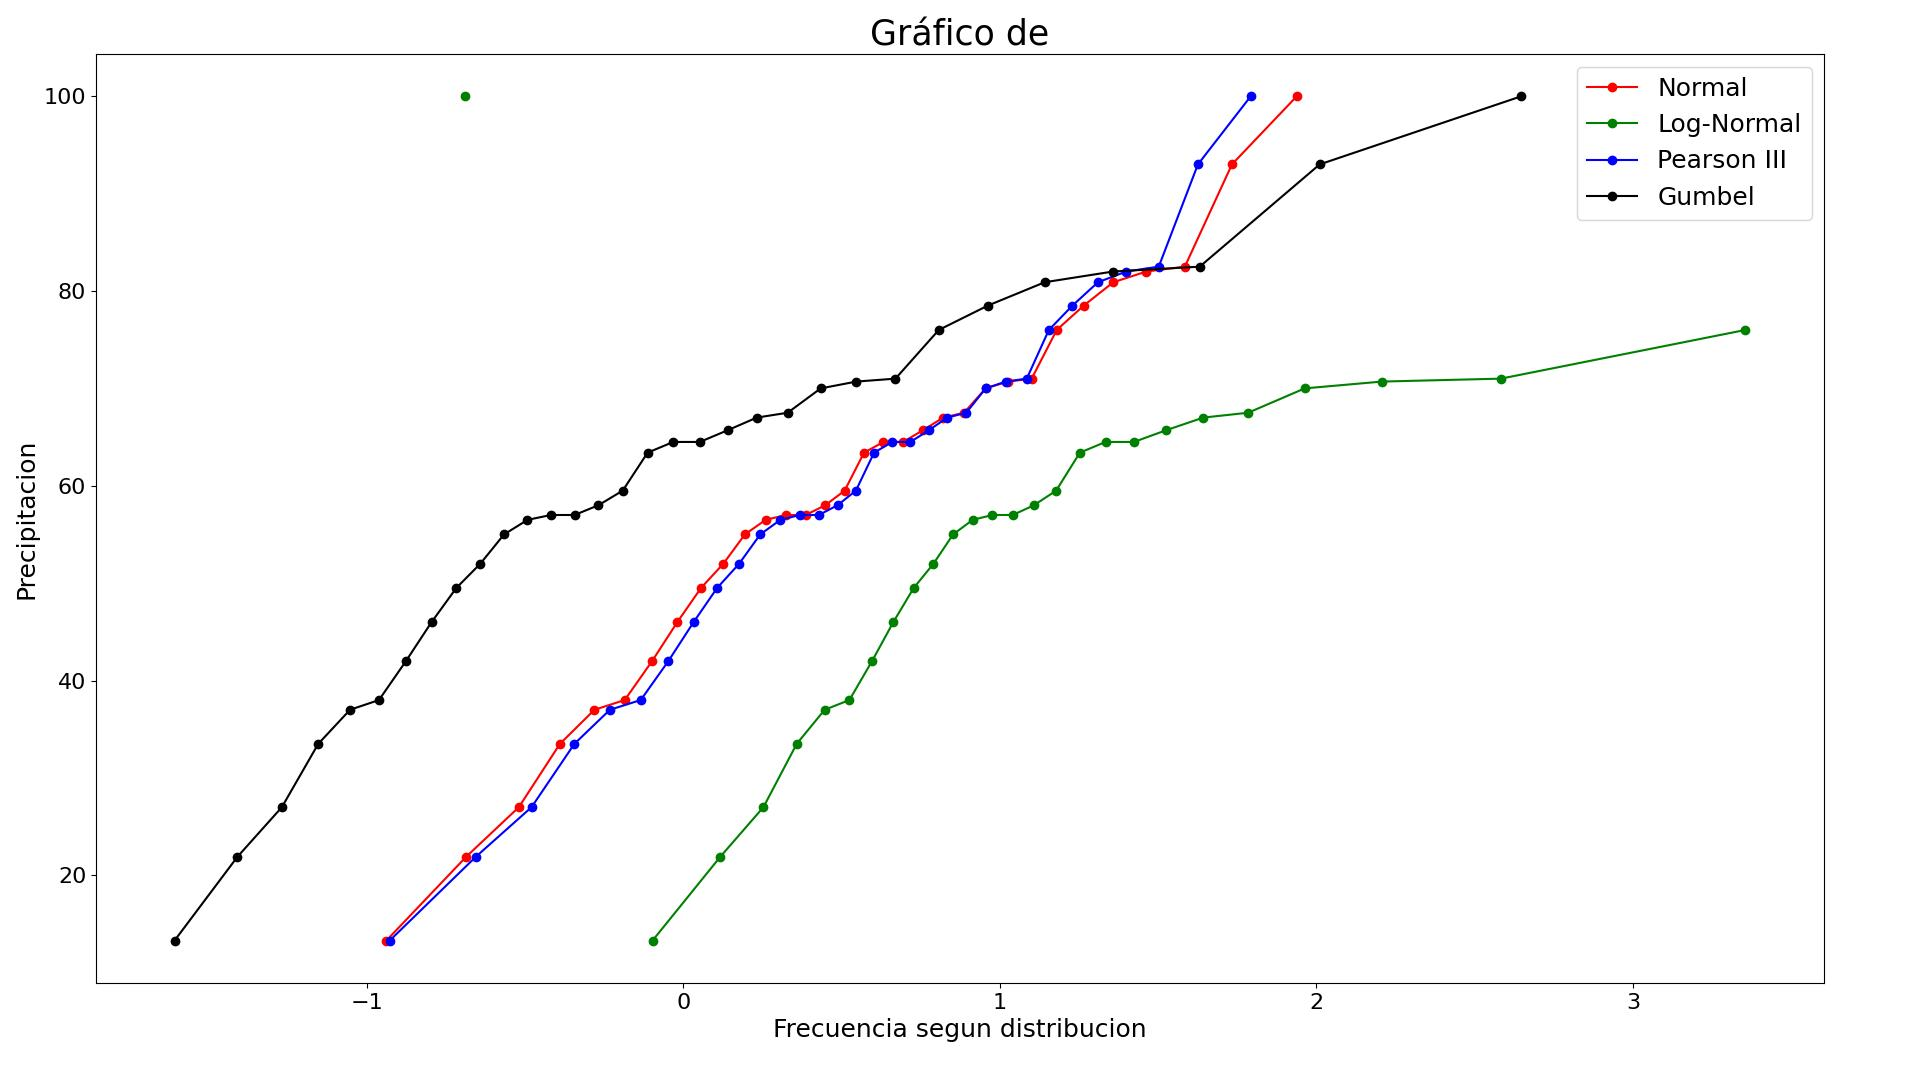
\includegraphics[width=0.8\textwidth]{grafico.jpg}
  \caption{Grafico de las frecuencias de precipitaciones segun las distintas distribuciones}
  \label{fig:grafico}
\end{figure}

\begin{figure}[H]
  \centering
  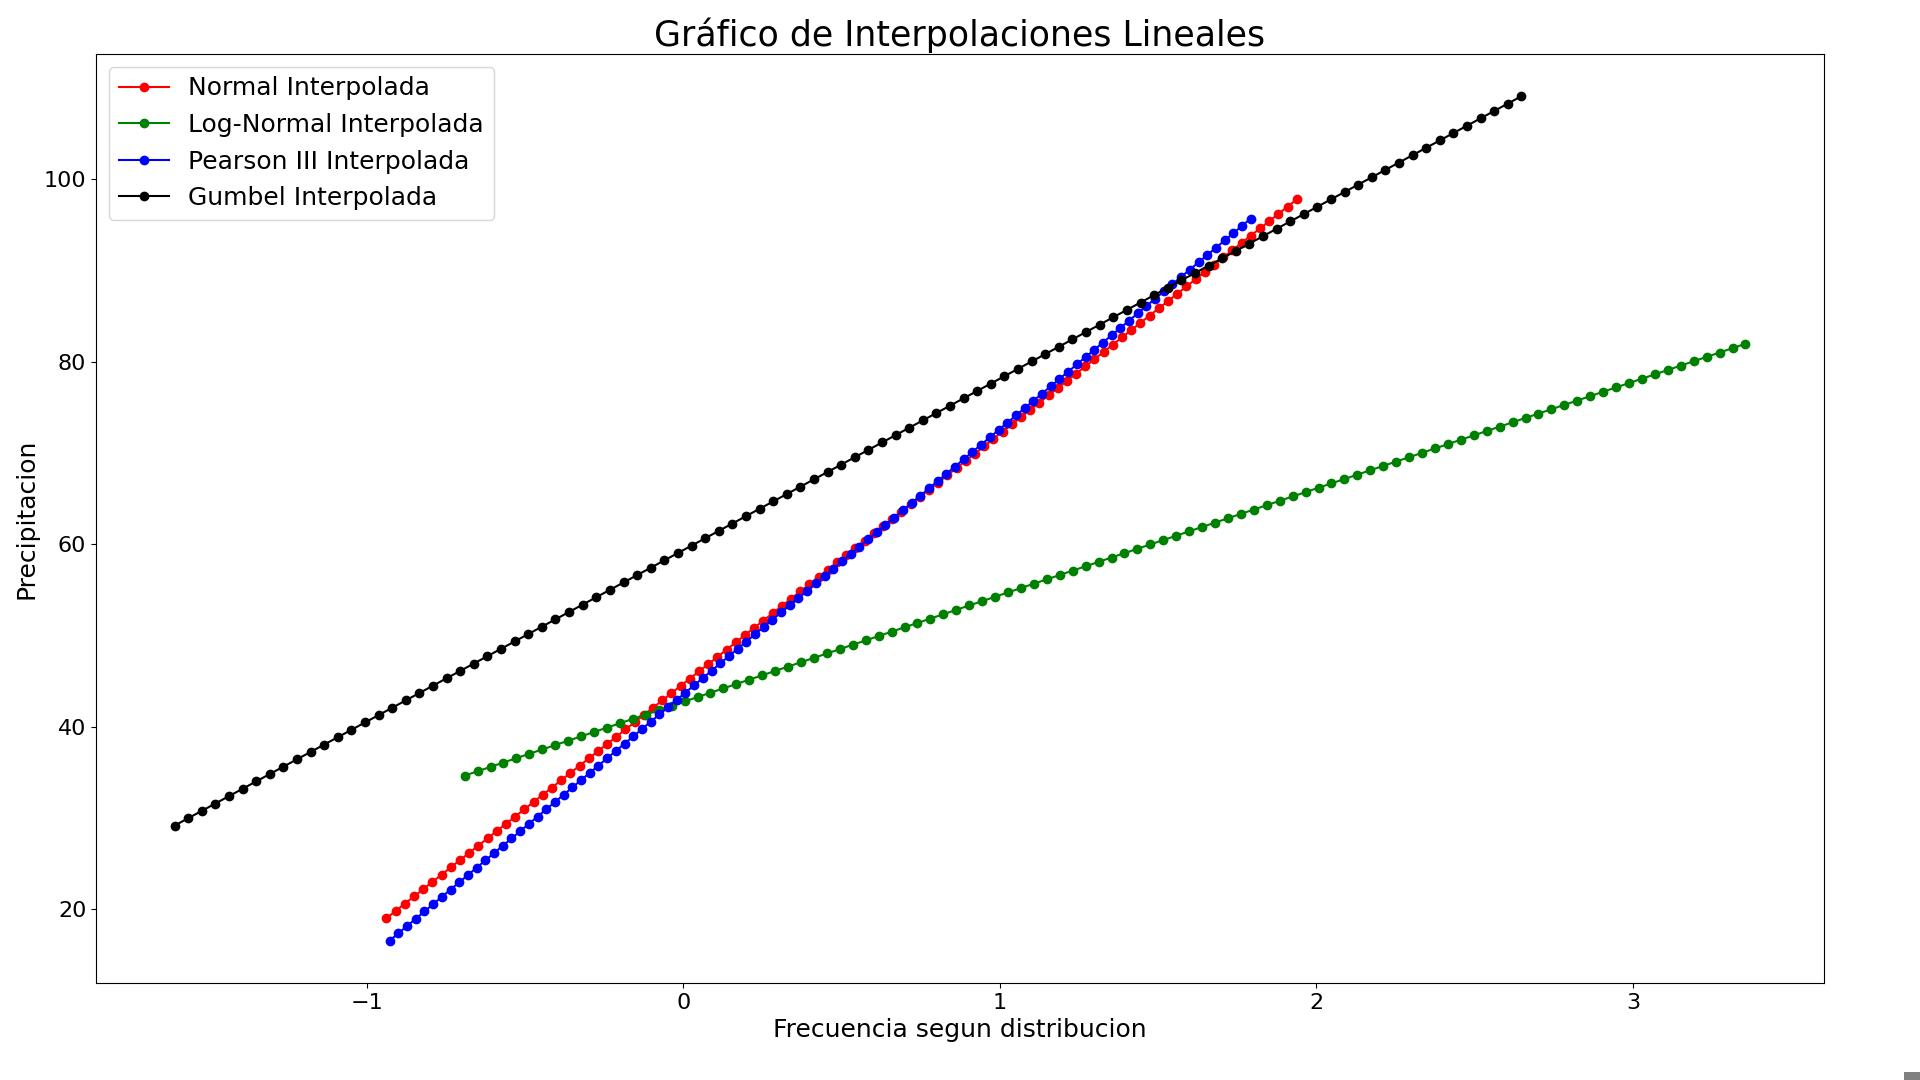
\includegraphics[width=0.8\textwidth]{grafico_interpolado.jpg}
  \caption{Grafico de las frecuencias de precipitaciones segun las distintas distribuciones interpoladas}
  \label{fig:grafico_interpolado}
\end{figure}

Los graficos \ref{fig:grafico} y \ref{fig:grafico_interpolado} muestran las frecuencias de precipitaciones segun las distintas distribuciones. Ademas, se obtuvieron los siguientes valores para los coeficientes \( K_t \) y las precipitaciones para diferentes periodos de retorno:

\begin{table}[H]
  \centering
  \caption{Valores de \( K_t \) para diferentes períodos de retorno}
  \begin{tabular}{|c|c|c|c|c|}
  \hline
  \textbf{Período de Retorno (T)} & \textbf{Normal} & \textbf{Log-Normal} & \textbf{Pearson} & \textbf{Gumbel} \\ \hline
  10 años  & 1.5455 & -3.2158 & 1.4692 & 1.5410 \\ \hline
  50 años  & 2.0358 & 1.0396 & 1.8709 & 3.0257 \\ \hline
  100 años & 2.1660 & 1.7478 & 1.9738 & 3.6533 \\ \hline
  200 años & 2.2627 & 2.3380 & 2.0492 & 4.2787 \\ \hline
  \end{tabular}
  \label{table:kt}
\end{table}

\begin{table}[H]
  \centering
  \caption{Valores de precipitación (mm) para diferentes períodos de retorno}
  \begin{tabular}{|c|c|c|c|c|}
  \hline
  \textbf{Período de Retorno (T)} & \textbf{Normal} & \textbf{Log-Normal} & \textbf{Pearson} & \textbf{Gumbel} \\ \hline
  10 años  & 87.07 & 5.07 & 86.31 & 88.33 \\ \hline
  50 años  & 100.51 & 54.88 & 98.00 & 116.24 \\ \hline
  100 años & 104.08 & 63.17 & 101.00 & 128.04 \\ \hline
  200 años & 106.73 & 70.08 & 103.19 & 139.80 \\ \hline
  \end{tabular}
  \label{table:precipitacion}
\end{table}

De los cuadros \ref{table:kt} y \ref{table:precipitacion} se puede observar que las precipitaciones aumentan a medida que el periodo de retorno esperado aumenta. Ademas, se puede observar que las precipitaciones para la distribución Log-Normal son menores que para las otras distribuciones.

\begin{figure}[H]
  \centering
  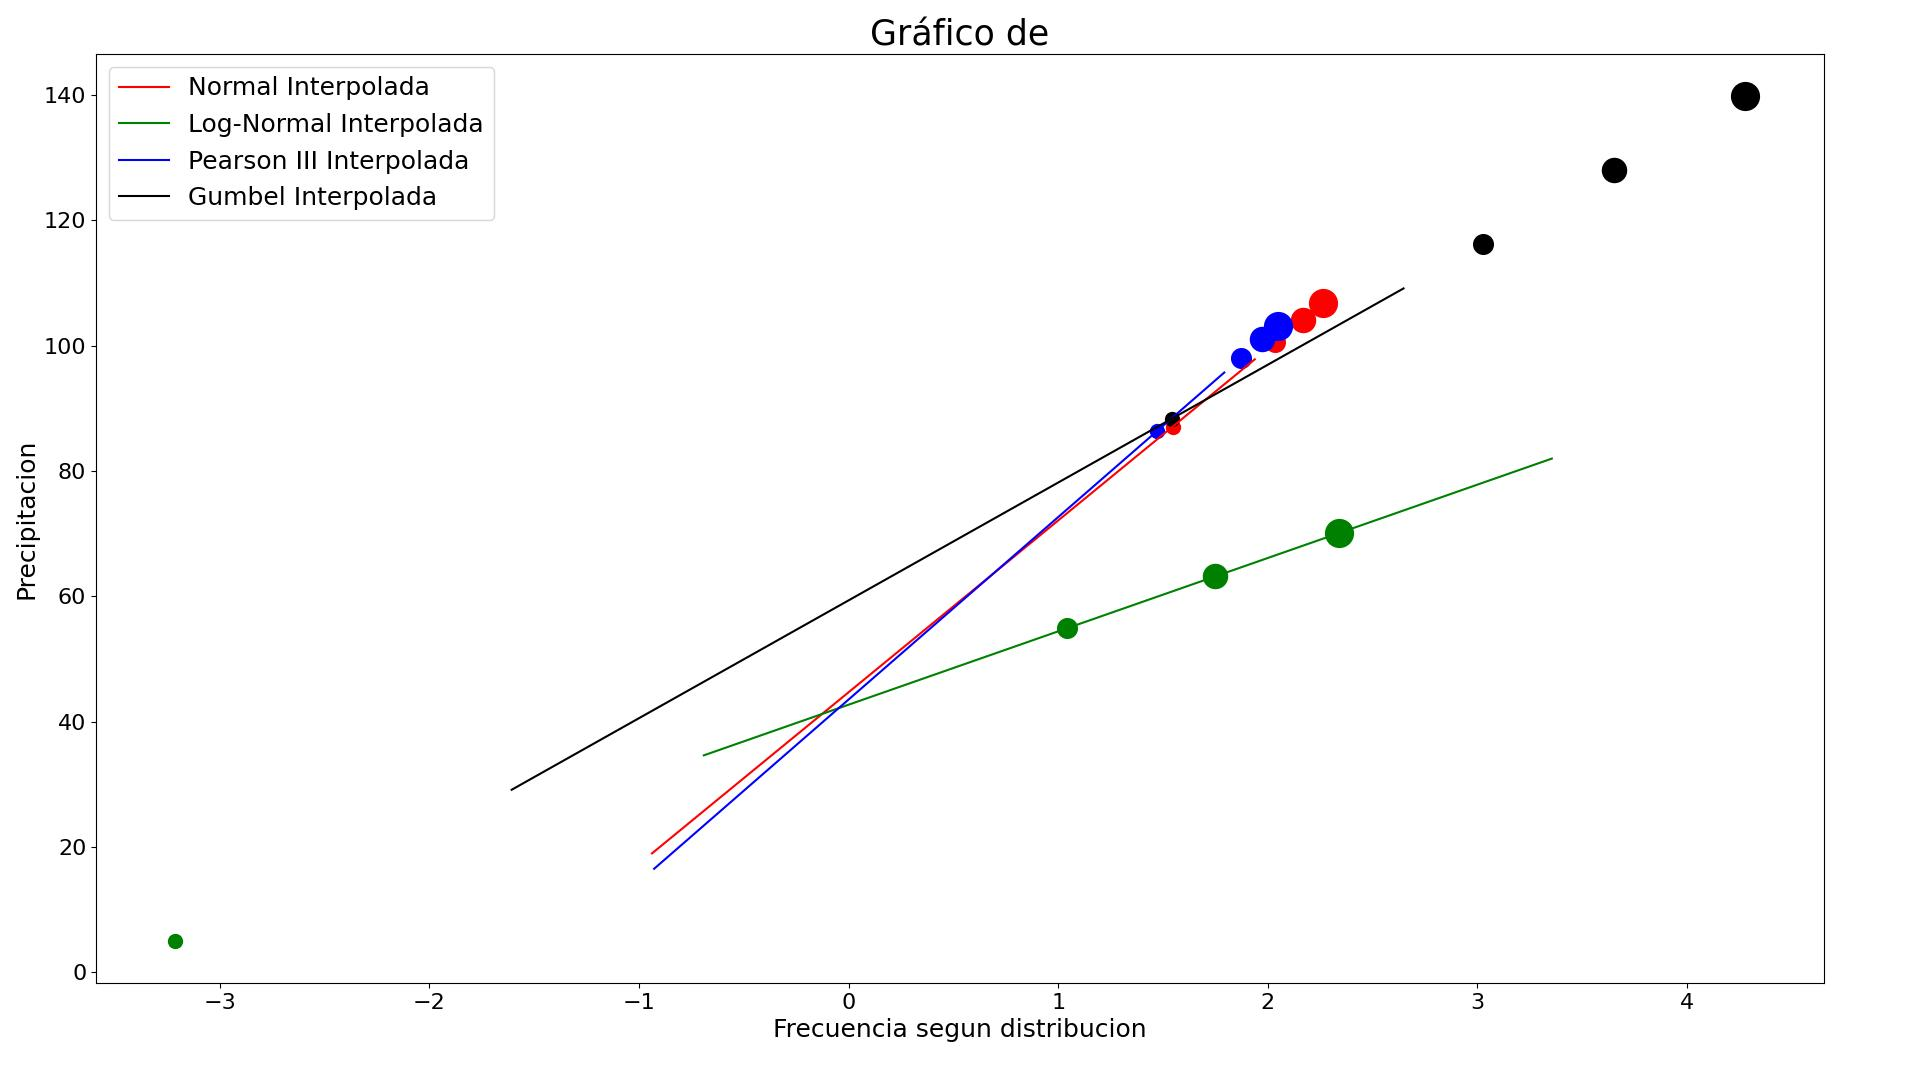
\includegraphics[width=0.8\textwidth]{grafico_proyecciones.jpg}
  \caption{Proyecciones de las frecuencias esperadas de precipitaciones para cada distribución}
  \label{fig:grafico_proyecciones}
\end{figure}

Finalmente, del grafico \ref{fig:grafico_proyecciones} se puede observar que las precipitaciones aumentan en el futuro, lo que se puede atribuir al cambio climatico.

\newpage
\subsubsection*{Parte B}

A continuación se presentan los resultados obtenidos en el caso de las proyecciones futuras (2040-2069) para la estación de San José de Maipo, con las distribuciones Normal, Log-Normal, Pearson III y Gumbel:

\begin{figure}[H]
  \centering
  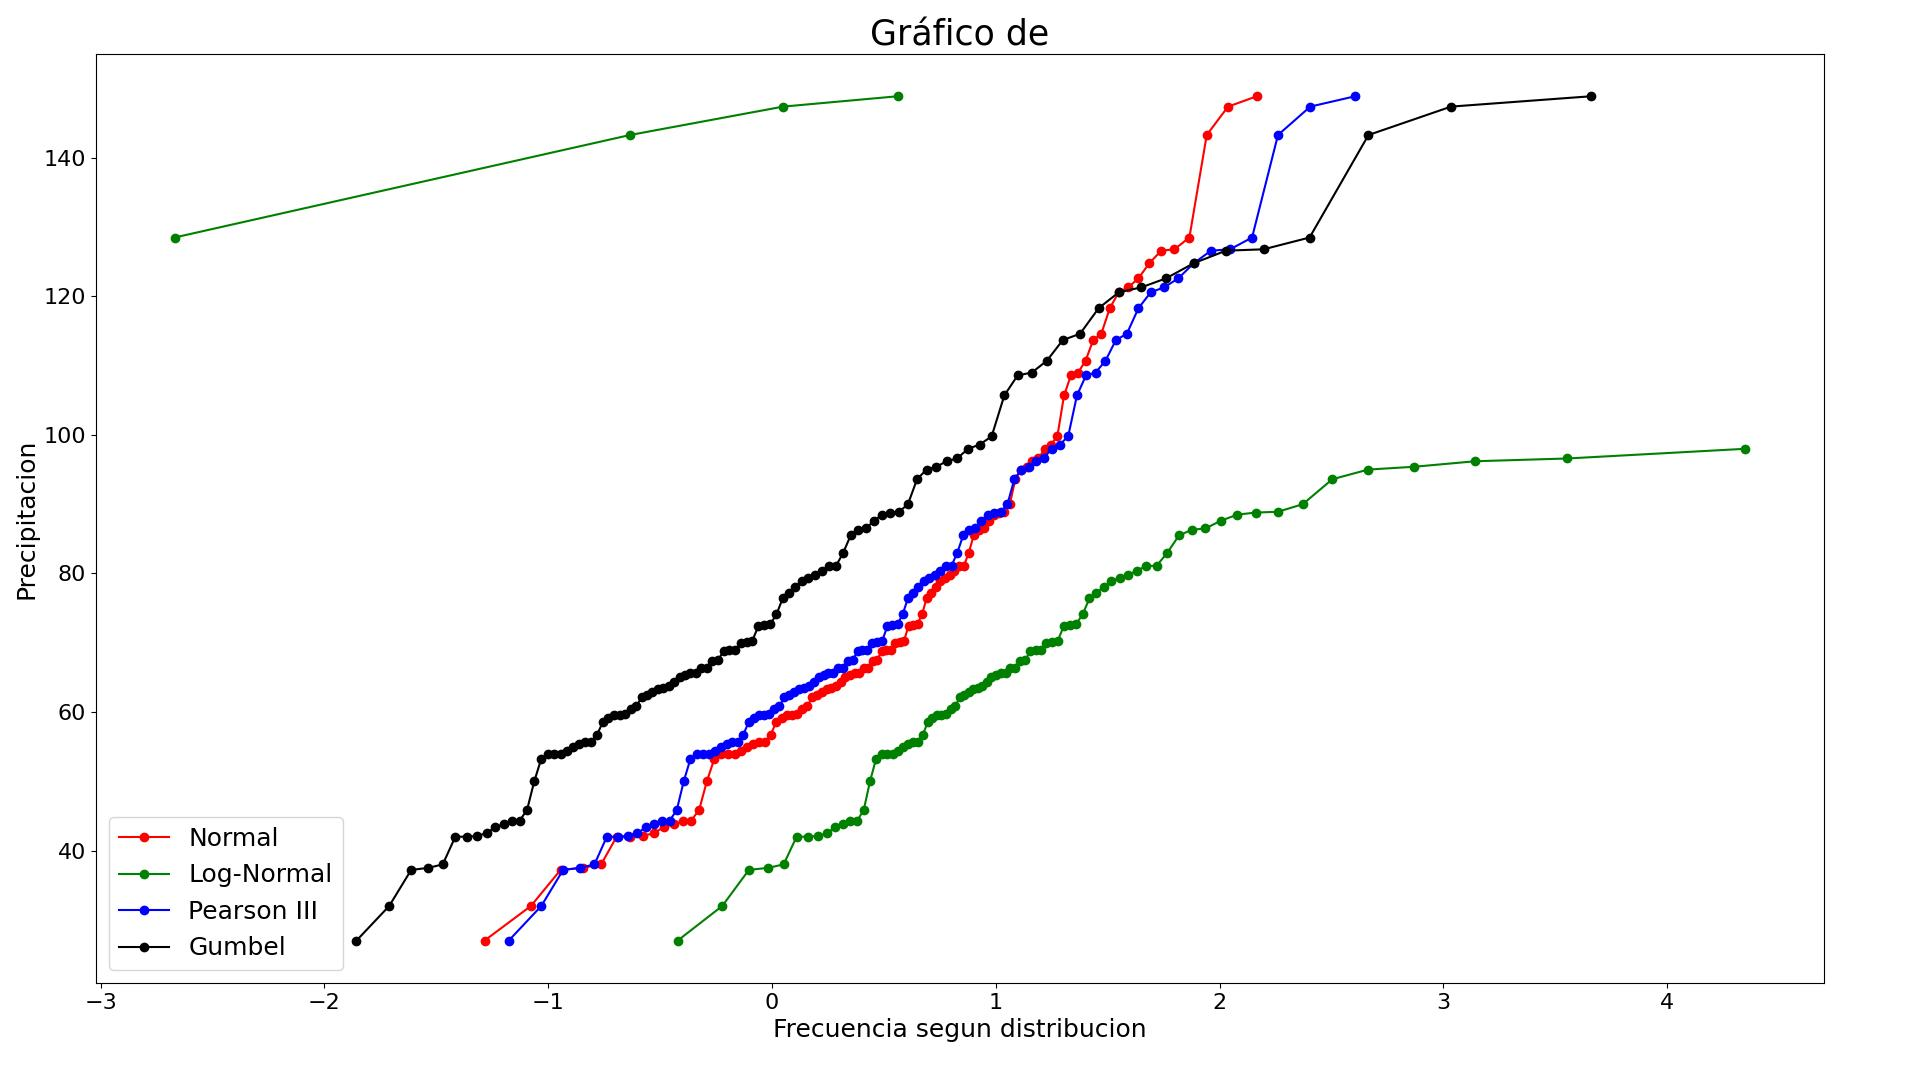
\includegraphics[width=0.8\textwidth]{grafico_b.jpg}
  \caption{Grafico de las frecuencias de precipitaciones segun las distintas distribuciones}
  \label{fig:grafico_b}
\end{figure}

\begin{figure}[H]
  \centering
  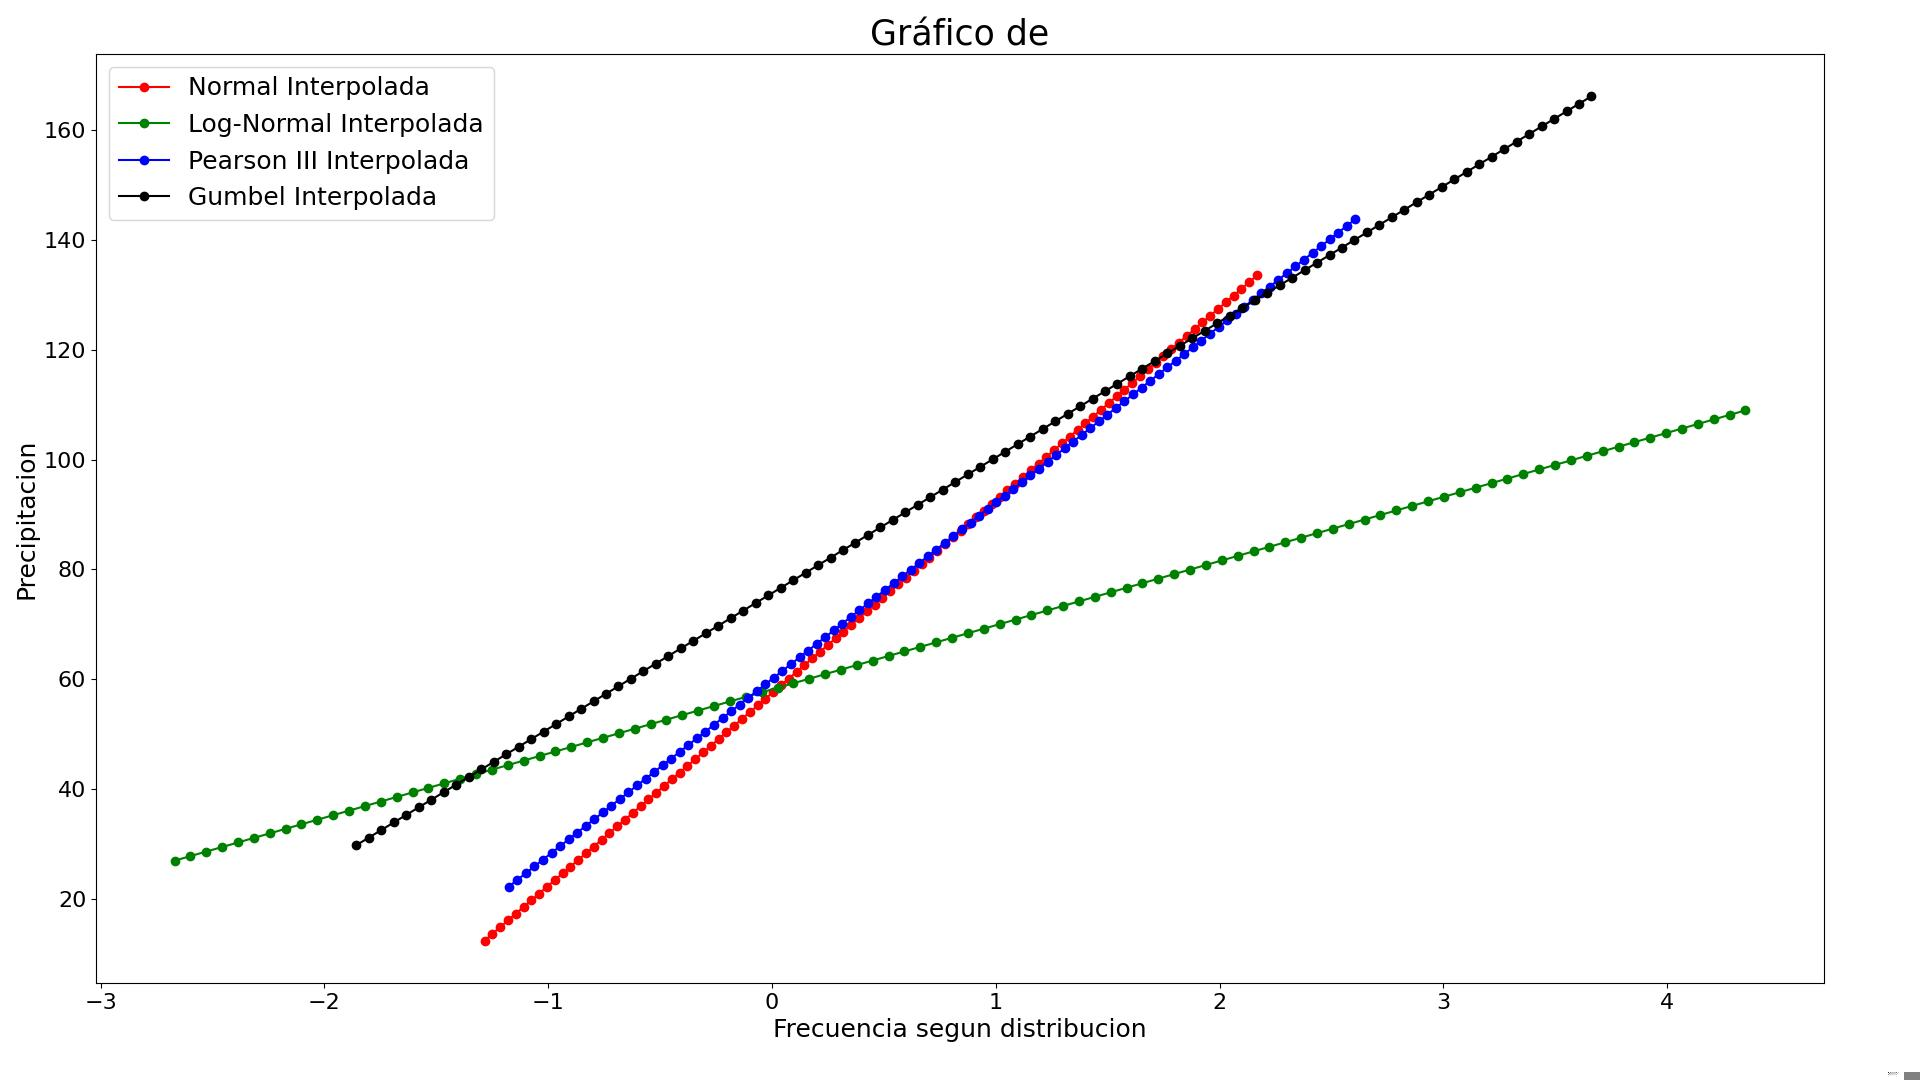
\includegraphics[width=0.8\textwidth]{grafico_b_interpolado.jpg}
  \caption{Grafico de las frecuencias de precipitaciones segun las distintas distribuciones interpoladas}
  \label{fig:grafico_b_interpolado}
\end{figure}

Los graficos \ref{fig:grafico_b} y \ref{fig:grafico_b_interpolado} muestran las frecuencias de precipitaciones segun las distintas distribuciones. Ademas, se obtuvieron los siguientes valores para los coeficientes \( K_t \) y las precipitaciones para diferentes periodos de retorno:

\begin{table}[H]
  \centering
  \caption{Valores de \( K_t \) para diferentes períodos de retorno esperados para 2040-2069}
  \begin{tabular}{|c|c|c|c|c|}
  \hline
  \textbf{Período de Retorno (T)} & \textbf{Normal} & \textbf{Log-Normal} & \textbf{Pearson} & \textbf{Gumbel} \\ \hline
  10 años  & 1.55 & -3.22 & 1.69 & 1.54 \\ \hline
  50 años  & 2.04 & 1.04  & 2.40 & 3.03 \\ \hline
  100 años & 2.17 & 1.75  & 2.60 & 3.65 \\ \hline
  200 años & 2.26 & 2.34  & 2.76 & 4.28 \\ \hline
  \end{tabular}
  \label{table:kt_b}
\end{table}

\begin{table}[H]
  \centering
  \caption{Valores de precipitación (mm) para diferentes períodos de retorno esperados para 2040-2069}
  \begin{tabular}{|c|c|c|c|c|}
  \hline
  \textbf{Período de Retorno (T)} & \textbf{Normal} & \textbf{Log-Normal} & \textbf{Pearson} & \textbf{Gumbel} \\ \hline
  10 años  & 111.72 & 20.55 & 114.25 & 113.77 \\ \hline
  50 años  & 128.93 & 70.28 & 137.24 & 150.47 \\ \hline
  100 años & 133.50 & 78.56 & 143.73 & 165.99 \\ \hline
  200 años & 136.90 & 85.46 & 148.67 & 181.45 \\ \hline
  \end{tabular}
  \label{table:precipitacion_b}
\end{table}

De los cuadros \ref{table:kt_b} y \ref{table:precipitacion_b} se puede observar que las precipitaciones aumentan a medida que el periodo de retorno esperado aumenta. Ademas, se puede observar que las precipitaciones para la distribución Log-Normal son menores que para las otras distribuciones.

\begin{figure}[H]
  \centering
  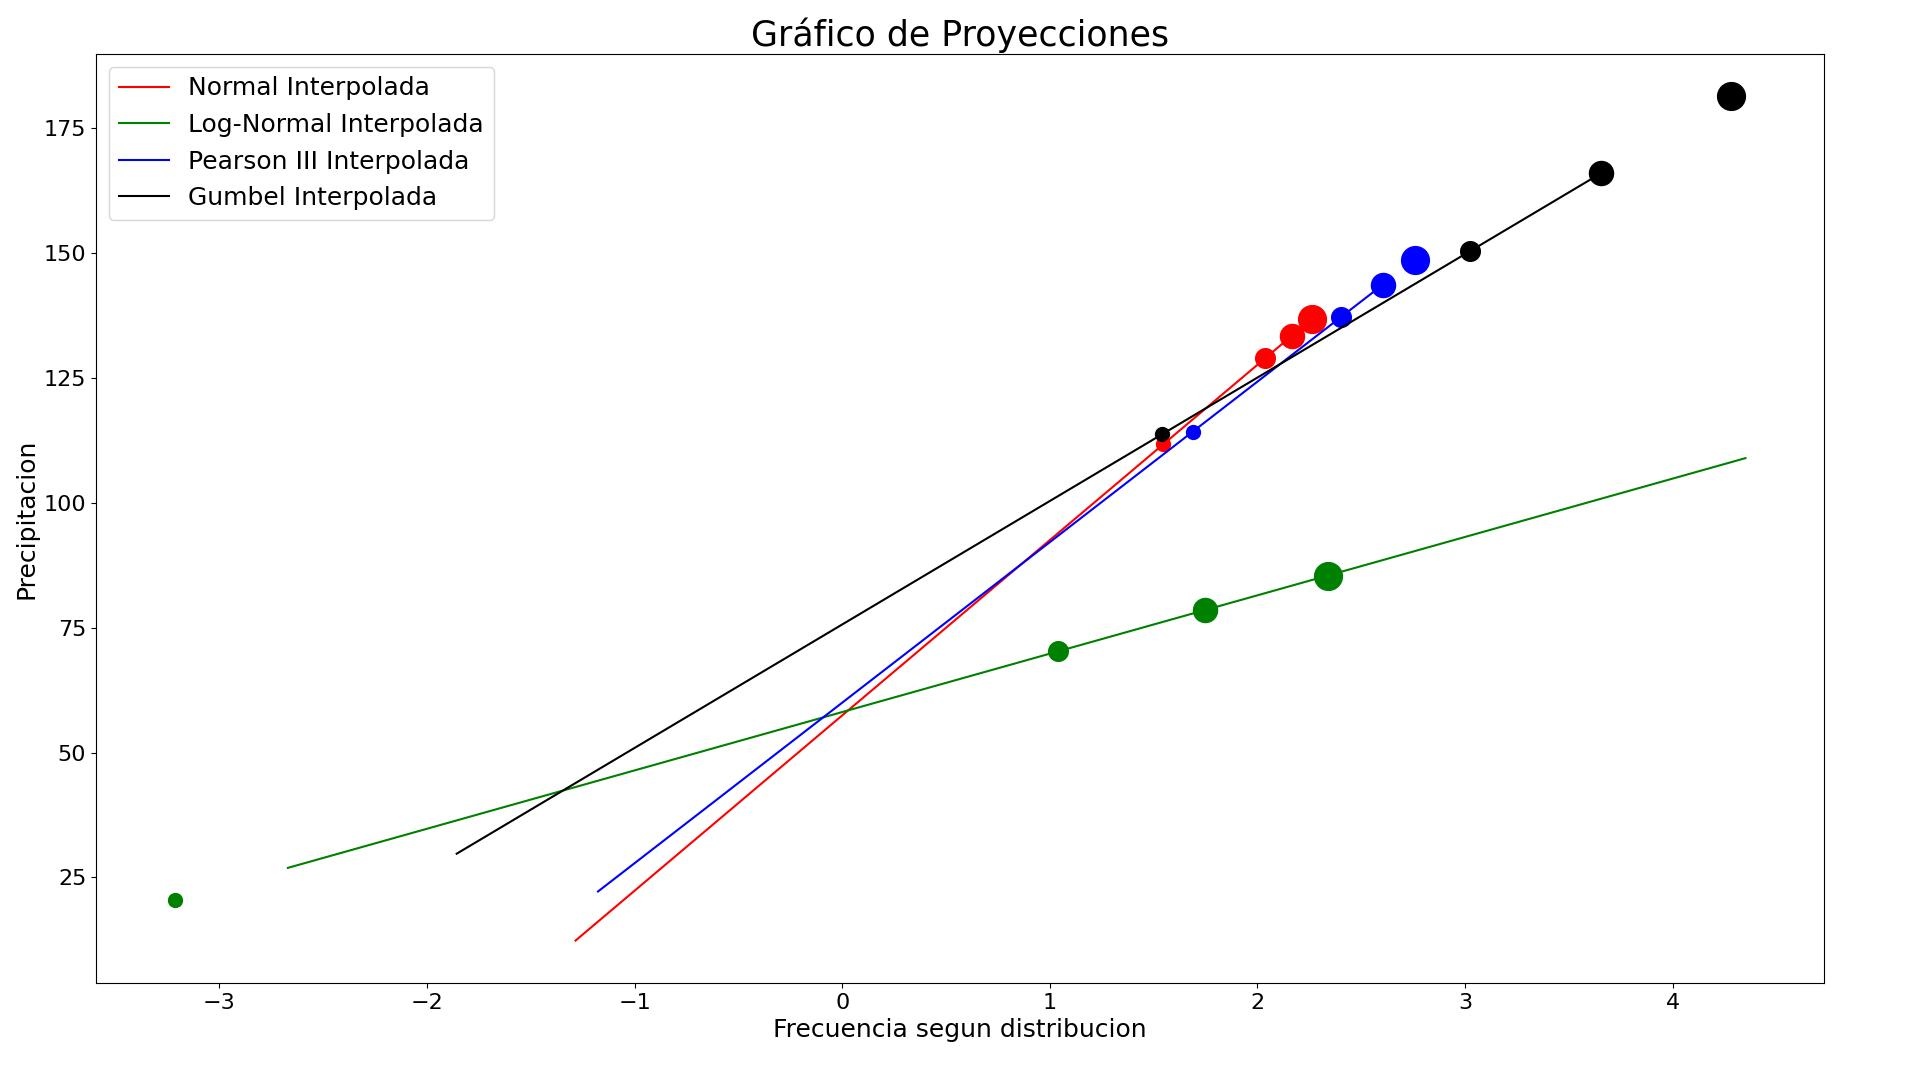
\includegraphics[width=0.8\textwidth]{grafico_b_proyecciones.jpg}
  \caption{Proyecciones de las frecuencias esperadas de precipitaciones para cada distribución}
  \label{fig:grafico_b_preyecciones}
\end{figure}

Finalmente, del grafico \ref{fig:grafico_b_preyecciones} se puede observar que las precipitaciones aumentan en el futuro, lo que se puede atribuir al cambio climatico y que no se esper que este deje de cambiar como lo esta haciendo ahora.

\subsubsection*{Parte C}

En este caso se compararan los datos obtenidos en las partes A y B, para entender como el paso del tiempo afecta las precipitaciones máximas de la zona. \\

A continuación se presentan las diferencias en las precipitaciones máximas estimadas para los períodos de retorno considerados (10, 50, 100, 200 años) entre las partes A (histórico) y B (futuro):

\begin{table}[H]
  \centering
  \caption{Comparación de precipitaciones (mm) para diferentes períodos de retorno}
  \begin{tabular}{|c|c|c|c|}
  \hline
  \textbf{Período de Retorno (T)} & \textbf{Histórico (1990-2021)} & \textbf{Futuro (2040-2069)} & \textbf{Porcentaje de cambio} \\ \hline
  10 años  & 87.07 & 111.72 & +28.33\% \\ \hline
  50 años  & 100.51 & 128.93 & +28.26\% \\ \hline
  100 años & 104.08 & 133.50 & +28.27\% \\ \hline
  200 años & 106.73 & 136.90 & +28.28\% \\ \hline
  \end{tabular}
  \label{table:comparacion_c}
\end{table}

Como se observa en la tabla \ref{table:comparacion_c}, las precipitaciones máximas proyectadas para los diferentes períodos de retorno, demuestran que con el paso del tiempo las ptrcipitaciones aumenten en un 28.3\% aproximadamente para todos los períodos de retorno. 

Es válido comparar los resultados de las partes A y B porque ambos análisis se enfocan en la misma zona (San José de Maipo) y utilizan métodos estadísticos similares para estimar las precipitaciones máximas. Sin embargo, es importante considerar que las proyecciones futuras provienen de modelos climáticos, que pueden tener algunas incertidumbres. Aun así, son útiles para anticipar posibles cambios en el clima extremo.

La mejor comparación para evaluar los cambios sería entre los resultados históricos y las proyecciones futuras, ya que esto muestra el impacto del cambio climático en las precipitaciones extremas. Este análisis es clave para planificar infraestructura y gestionar riesgos, ya que un aumento en las lluvias intensas podría provocar más inundaciones y otros problemas.

\newpage
\section{Conclusión}

El análisis realizado muestra que las precipitaciones máximas en San José de Maipo probablemente aumenten en el futuro debido al cambio climático, con un incremento cercano al 28\% en los próximos años. Este cambio es importante porque podría llevar a más riesgos de inundaciones y otros fenómenos extremos. Además, el aumento de temperatura afecta la cantidad de agua precipitable en la atmósfera, lo que confirma que el cambio climático influye tanto en la cantidad de lluvia como en la intensidad de los eventos extremos. \\
En este caso la interpolacion para el grafico \ref{fig:grafico_interpolado} y el \ref{fig:grafico_b_interpolado}, son una herramienta que permite un mas facil y mejor manejo de los datos para realizar estudios de estos. Además, cabe destacar que en el caso del factor de frecuencia, al este aumentar se puede observar un aumento de las precipitaciones. Es por esto que segun las distribuciones normales y Pearson III, se puede observar un aumento significativo al k comenzar a ser mayor a 1. \\
Este tipo de analisis son fundamentales para la plinificacion de infraestructuras y la gestion de riesgos, ya que permiten anticipar posibles cambios en el clima y adaptarse a ellos. En este sentido, es importante llevar un monitoreo sobre el pasado y estimaciones sobre el futuro para asi poder tomar decisiones informadas y minimizar los impactos del cambio climático.

\end{document}
